The previous section demonstrates the RF modules that involve  the communication between PCD and PICC. This section will describe in detail each module of the analog front-end for ISO/IEC 14443A (see Fig. \ref{fig:afe}).

\begin{figure}[]
  \centering
  \includegraphics[page=10,width=80mm]{images-crop.pdf}
  \caption{PICC Analog Front-end}
  \label{fig:afe}
\end{figure}

\subsection{Power Supply Generator (PSG)}

The Power Supply Generator splits into two parts: signal rectification and power limitation.

The first part rectifies the RF field signal to get power supply for the chip, a full NMOS bridge rectifier \cite{rfid_rect1}\cite{rfid_rect2} was implemented in this design. And the second part consists of a Shunt resistor. The Shunt resistor is capable to limit the voltage of the antenna and protects the whole chip. ISO/IEC14443-2 requires the PICC to work when magnetic intensity between 1.5-7.5A/m rms. Therefore the PICC must work in these extreme conditions.  

The simplified schematic of signal rectification is shown in Fig. \ref{fig:rect} and power limitation (Shunt resistor) is shown in Fig. \ref{fig:shunt}.

\begin{figure}[h]
  \centering
  \includegraphics[page=11,width=60mm]{images-crop.pdf}
  \caption{Full Wave Rectifier}
  \label{fig:rect}
\end{figure}

\begin{figure}[h]
  \centering
  \includegraphics[page=12,width=60mm]{images-crop.pdf}
  \caption{Shunt Resistor}
  \label{fig:shunt}
\end{figure}

\subsection{Clock Generator (CG)}

The Clock Generator recovers the clock from the antenna and is used by the DPU. This module generates a clock source of 13.56 MHz. Basically consists of two FF/D (clock divider by 2) and a XOR logic gate. 

The difference of phase between RF+ and RF- are 180 degrees, it is easy to take advantage of this property to recompose the clock. The simplified schematic is shown in Fig. \ref{fig:clk} and the simulation in the Fig. \ref{fig:clk_sim}.

A frequency divider by 4 is placed at the output of the clock generator, reducing the work frequency also reduces the power consumed. On the other hand, Carrier-Frequency/4 (3.39MHz) is used for the DPU, because the FDT (Frame Delay Time)  defined in ISO/IEC14443-3 is for all commands are divisor of this frequency.
 

\begin{figure}[]
  \centering
  \includegraphics[page=13,width=60mm]{images-crop.pdf}
  \caption{Clock Generator schematic}
  \label{fig:clk}
\end{figure}

\begin{figure}[]
  \centering
  \includegraphics[page=14,width=80mm]{images-crop.pdf}
  \caption{Clock recovery simulation}
  \label{fig:clk_sim}
\end{figure}

\subsection{Voltage Regulator (VR)}

The Voltage Regulator \cite{rfid_ldo} regulates the voltage supplied from PSG and provide a constant DC voltage at the output of this module. The VR is known as the series pass regulator, as shown in Fig. \ref{fig:ldo}. It consists of 3 major parts. Operational amplifier (OP-AMP) is used as error amplifier. A series pass transistor forms a current amplifier. R1 and R2 are used as resistive voltage divider (Ecuation \ref{eq:vref}). The reference source Vref, in this case, is a beta multiplier \cite{panadero}. 

\begin{equation} \label{eq:vref}
VDD = Vref*(1+R1/R2)
\end{equation}
%$$VDD = Vref*(1+R1/R2)$$  

%Basically it consist of a reference source, in this case, a beta multiplier is used for this purpose. The OP AMP play the role of controller, it copies the reference voltage, control the variation of VRECT or VDD and reflects the reference voltage to the output.

\begin{figure}[]
  \centering
  \includegraphics[page=15,width=60mm]{images-crop.pdf}
  \caption{Voltage Regulator schematic}
  \label{fig:ldo}
\end{figure}

\subsection{Modulator}

The modulator \cite{rfid_modulador} transmits the signal from PICC to PCD. There are two different types of load modulation: resistive and capacitive modulation. Both types create a subcarrier next to 13.56MHz. The NMOS are switched on and off in time with the encoded data. This will vary the load (resistive) or resonance frequency  (capacitive) of the transponder.  Resistive modulation was adopted in this design for its simplicity. The schematic is shown in Fig. \ref{fig:mod}.

\begin{figure}[h]
  \centering
  \includegraphics[page=16,width=40mm]{images-crop.pdf}
  \caption{Modulator schematic}
  \label{fig:mod}
\end{figure}

\subsection{Demodulator}

The demodulator recovers the digital signals from the ASK signal transmitted from PCD. An Envelope Extractor (EE) \cite{rfid_demodulador} is needed to extract the data. The digital signal is recovered by connecting the output of the EE with the input of the buffer. The circuit is shown in Fig. \ref{fig:demod}. 

\begin{figure}[h]
  \centering
  \includegraphics[page=17,width=80mm]{images-crop.pdf}
  \caption{Demdulator schematic}
  \label{fig:demod}
\end{figure}

\subsection{Power On Reset (POR)}

The Power On Reset module is used to reset the digital machine and put it into idle state. It consists of a RC low pass network. When the chip enter to the RF field, the VR turns on and power all the modules. The POR module holds the voltage of the VR and delays it. This signal applies to the reset pin of the Flip-Flops in the digital machine. The schematic is demonstrated in Fig. \ref{fig:por}. 

\begin{figure}[h]
  \centering
  \includegraphics[page=18,width=20mm]{images-crop.pdf}
  \caption{POR schematic}
  \label{fig:por}
\end{figure}